\def\QRCODE{TB_image_TUT.IMG.cornea_fourier_matlabqrcode.png}
\def\QRPAGE{http://www.iptutorials.science/tree/master/TB_image/TUT.IMG.cornea_fourier/matlab}
\mcorrectionsection{Matlab correction}

\subsection{Fourier transform}

In order to display the Fourier transform, the following function is used to show both spectrum and phase. Notice the logarithmic function.

\begin{matlab}
function viewImageSpectrum(I,F)
% I: original image
% F: Fourier transform of I

subplot(1,3,1);
imshow(I,[]);

% phase
subplot(1,3,3);
Im=angle(S);
imshow(Im,[]);

% amplitudes
subplot(1,3,2);
Ia=abs(S);
Ia2=log(1+Ia);
imshow(Ia2,[]);
\end{matlab}

The \minline{fftshift} functions centers the frequency $(0,0)$ in the image. The following functions will be used:
\begin{matlab}
% Fourier transform utility of image I
function S=FT(I)
S=fftshift(fft2(double(I)));
\end{matlab}

\begin{matlab}
% Inverse Fourier transform utility of spectrum S
function I=iFT(S)
I=real(ifft2(fftshift(S)));
\end{matlab}

\subsection{Inverse Fourier Transform}
The important thing to notice in the 2D Fourier transform is that the information is present in the phase, not in the amplitude. The following code highlights this property (see also Fig.\ref{fig:fourier:matlab:partial}).

\begin{matlab}
Spectrum=FT(A);

% amplitude and phase
amplitude = abs(Spectrum);
phase = angle(Spectre);

% reconstruction with amplitude only
C=real(ifft2(fftshift(amplitude)));
figure;imshow(C,[]);title('Reconstruction from amplitude only');

% reconstruction with phase only
D=real(ifft2(fftshift((exp(1i*phase)))));
figure;imshow(D,[]);title('Reconstruction from phase only');
\end{matlab}

\begin{figure}[htbp]
 \centering
 \subfloat[Amplitude on\-ly.]{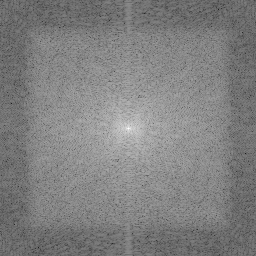
\includegraphics[width=6cm]{amplitude_brain.png}}
 \hspace{1cm}
 \subfloat[Phase only.]{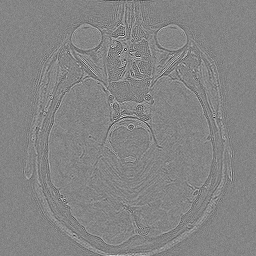
\includegraphics[width=6cm]{phase_brain.png}}
 \caption{Reconstruction of partial informations (phase or amplitude only). Notice that the main visual informations are contained in the phase, and not in the amplitude.}
 \label{fig:fourier:matlab:partial}
\end{figure}

\subsection{Low-pass and high-pass filtering}
This is done by selecting only low or high frequencies, respectively. A binary window is employed.
\begin{figure}[htbp]
 \centering
 \subfloat[High Pass filter.]{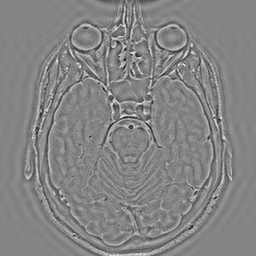
\includegraphics[width=6cm]{highpass_brain.png}}
 \hspace{1cm}
 \subfloat[Low Pass filter.]{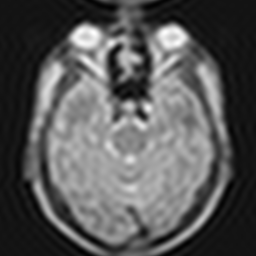
\includegraphics[width=6cm]{lowpass_brain.png}}
 
 \subfloat[Filtering (binary) mask.]{\fbox{
\includegraphics[width=4cm]{filter.png}}}
 \caption{Fourier basic filtering of the brain image.}
 \label{fig:fourier:matlab:filters}
\end{figure}

\begin{matlab}
function Sr=LPfilter(S, fC)
% low pass filtering
% S: spectrum (Fourier Transform)
% fC: cut-off frequency
fC=floor(fC);
if(fC<=0 | 2*fC >= size(S,2) | 2*fC >= size(S,1) )
   disp('Wrong cut-off frequency');
   Sr=0;
   return;
end

So=zeros(size(S));
So((size(S,1)/2-fC):(size(S,1)/2+fC), (size(S,2)/2-fC):(size(S,2)/2+fC))=1;
Sr=S.*So;
\end{matlab}

\begin{matlab}
function Sr=FiltrePH(S, fC)
% High pass filter
% S: spectrum (fourier transform)
% fC: cut-off frequency

fC=floor(fC);
if(fC<=0 | 2*fC >= size(S,2) | 2*fC >= size(S,1) )
   disp('Taille de coupure incorrecte');
   Sr=0;
   return;
end

So=ones(size(S));
So((size(S,1)/2-fC):(size(S,1)/2+fC), (size(S,2)/2-fC):(size(S,2)/2+fC))=0;
Sr=S.*So;
\end{matlab}

The two previous functions are used to filter the image, which is done with:
\begin{matlab}
Spectre_PB0=FiltrePB(Spectrum,20);
Spectre_PH0=FiltrePH(Spectrum,110);
% inverse Fourier transform
A_PB0=iFT(Spectre_PB0);
A_PH0=iFT(Spectre_PH0);
% display results
viewImageSpectre(A_PB0,Spectre_PB0);title('Low-pass filter');
viewImageSpectre(A_PH0,Spectre_PH0);title('High-pass filter');
\end{matlab}

\subsection{Application: evaluation of corneal cell density}
The principle consists in isolating the annulus (see Fig.\ref{fig:fourier:matlab:amplitude_cornea}) that corresponds to a frequency of repetition of the cells, that can lead us to a cell density. First of all, the image is loaded and the FFT is applied.

\begin{matlab}
A=imread('cornee.tif');
% spectrum
Spectrum=FT(A);
% amplitude and phase computation
amplitude = abs(Spectrum);
phase = angle(Spectrum);
\end{matlab}

\begin{figure}[htbp]
 \centering
 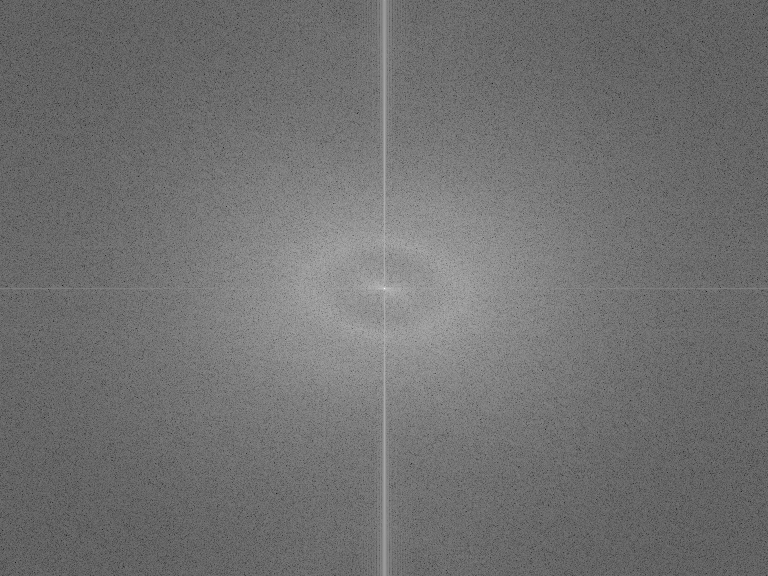
\includegraphics[width=.5\linewidth]{FT_cornea.png}
 \caption{Amplitude of the spectrum of the cornea image. Notice the circular shape that denotes a certain regularity of the cellular pattern, and can be used in order to evaluate the cell density.}
 \label{fig:fourier:matlab:amplitude_cornea}
\end{figure}


Then, the amplitude is filtered. A central line is kept. The objective is now to extract the second peak. The results of the \minline{findpeaks} function are displayed in Fig.\ref{fig:fourier:matlab:peaks}.

\begin{matlab}
% Filtering of 
PSF = fspecial('gaussian',30,30);
Blurred = imfilter(amplitude,PSF,'symmetric','conv');

V = Blurred(:,end/2);
plot(V);

% In order to find the peaks, the method is elementary:
% we are looking for the 2nd peak, at length(V)/2
[pks, locs] = findpeaks(V);
hold on
plot(locs, pks, 'sr');
locs2 = sort(abs(length(V)/2-locs))

% result is displayed
disp('frequency of repetition:')
f=locs2(2)/length(V)
disp('cornea diameter:')
d=1/f
\end{matlab}

\begin{mwindow}
locs2 =
     1
    49
    50
   200
   214
   224
   225
   234
   274
   277
   281
   281
   284
   285
   286

frequency of repetition:
f =
    0.0851

cornea diameter:
d =
   11.7551
>>
\end{mwindow}

More informations can be see in \cite{Ruggeri2005,Grisan2005,Ruggeri2007,Selig2015}.

\begin{figure}[htbp]
\centering
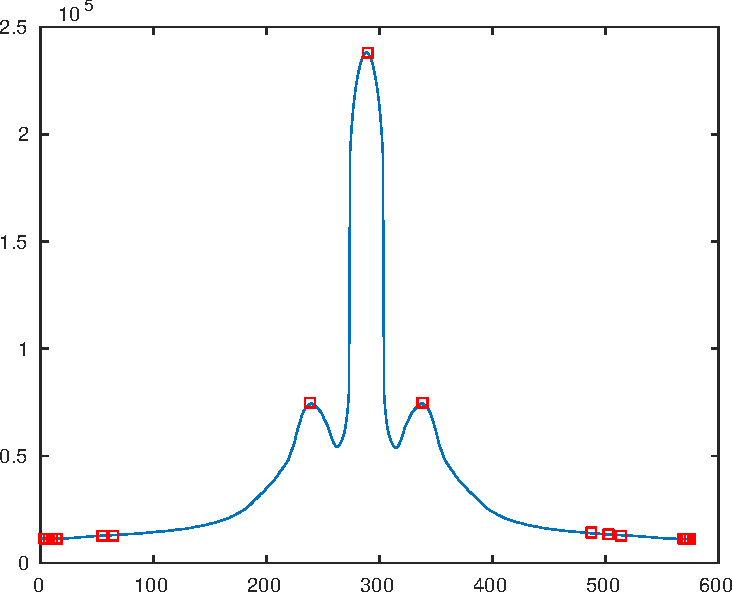
\includegraphics[width=10cm]{peaks.pdf}
 \caption{Detected peaks.}
 \label{fig:fourier:matlab:peaks}
\end{figure}
